\documentclass[12pt,a4paper]{article}

% Margins.
\setlength{\oddsidemargin}{0in}
\setlength{\evensidemargin}{0in}
\setlength{\headheight}{12pt}
\setlength{\headsep}{42pt}
\setlength{\topmargin}{-54pt}
\setlength{\textwidth}{6.5in}
\setlength{\textheight}{10in}

\usepackage{amsmath}
\usepackage{float}
\usepackage{graphicx}
\usepackage[hyphens]{url}
\usepackage{hyperref}	% Clickable links to figures, references and urls.
\usepackage{datetime}
\usepackage{longtable}
\usepackage{subfigure}

% Links direct to top of figures.
\usepackage[all]{hypcap}

% Drawing.
\usepackage{pgf}
\usepackage{tikz}

% Listings for formatting code.
\usepackage{listings}
\usepackage{textcomp}
% General options.+++
\lstset{breaklines=true, basicstyle=\small\ttfamily, tabsize=4, numbers=left, stepnumber=1, frame=single, showstringspaces=false, upquote=true}
% C++ specific high-lighting. Comments are 50/50 shades of green/black and strings coloured with 60/40 red/black mixture.
\lstset{language=[ISO]C++, commentstyle=\color{green!50!black}, keywordstyle=\color{blue}, stringstyle=\color{red!60!black}}

%opening
\title{\vspace{-3cm}Physics for Engineers\\Class 34\\Current Density}
\author{Attique Dawood}
\date{November 11, 2013\\[0.2cm] Last Modified: \today, \currenttime}
\begin{document}
\maketitle
\section{Announcements}
\begin{itemize}
\item Assignment 07 is due today.
\item Quiz \#07 today.
\item Expect assignment 08 shortly.
\end{itemize}
\section{Current Density}
It is useful to define current density as current passing or cutting through a cross--sectional area. Current density is denoted by \textbf{J} and is a vector quantity. Current density also gives the direction of current flow. Mathematically
\begin{equation}
I=\int\limits_{S}\textbf{J}\cdot d{\textbf{S}}.
\end{equation}
If a wire of radius $r$ carries a current $I$ then cross--sectional area of wire is $\pi r^2$ and
\begin{equation}
J=\dfrac{I}{\pi r^2}
\end{equation}
where
\begin{equation}
I=J\times\pi r^2.
\end{equation}
\newpage
\section{Exercises}
\noindent\textbf{Question 1} A wire of radius $0.1$ cm carries $5$ mA current. Find current density.\\[0.2cm]
\noindent\textbf{Question 2} A coaxial wire of inner radius $\rho<0.1$ cm carries $I=10$ mA current. The outer conductor exists at $0.2<\rho<0.25$ cm and carries 10 mA return current. Find current densities in inner and outer conductor.\\[0.2cm]
\begin{minipage}{0.5\textwidth}
\begin{figure}[H]
\centering
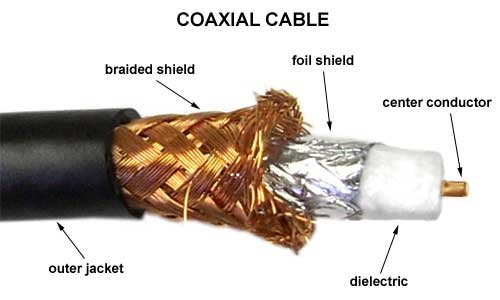
\includegraphics[scale=0.45]{CoaxialCable01.jpg}
\caption{Coaxial cable \cite{Ref:CoaxialCable01}.}
\label{Coaxial-cable}
\end{figure}
\end{minipage}
\begin{minipage}{0.5\textwidth}
\begin{figure}[H]
\centering
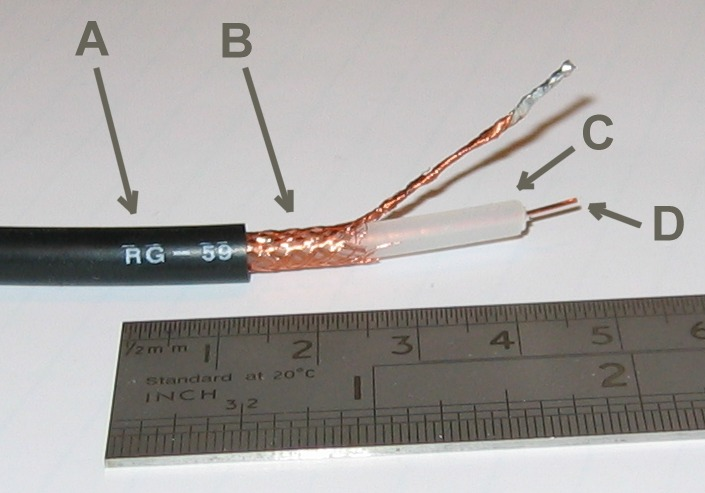
\includegraphics[scale=0.325]{CoaxialCable02.jpg}
\caption{RG-59 Coaxial cable \cite{Ref:CoaxialCable02}.}
\label{Coaxial-cable-rg59}
\end{figure}
\end{minipage}
%\nocite{*}
\bibliographystyle{plain}
\bibliography{PhysicsRef}
\end{document}
